\chapter{Arduino Startup}
\chaplabel{arduino}

\section{Installing the IDE}
We want to try using the IDE at least two different ways. First, on the lab computer, then on your personal
computers if you have them. 

\subsection{Lab Computer}
\begin{enumerate}
    \item On the search bar, type in Arduino. It should come up with Arduino IDE. 
    \item Click on Arduino IDE
    \item A script (DOS prompt) may appear for a bit. 
    \item After what could seem like a long time, the Arduino IDE should load.
    \item It should load up with a window that looks like Figure \ref{fig:emptysketch}.
    \item You will likely be prompted to upgrade the IDE since the installed software lags 
            behind the latest version a bit. It shouldn't matter if you use the installed 
            version and do not upgrade.
\end{enumerate}

\begin{figure}[!htb]
	\centering
	\includegraphics[scale=0.4]{arduinoStart/emptysketch.PNG}
	\caption{This is what the Arduino IDE should look like when it loads.}
	\label{fig:emptysketch}
\end{figure} 

\subsection{Personal Computer}
\begin{enumerate}
	\item Go to software download page: \href{https://www.arduino.cc/en/software}{https://www.arduino.cc/en/software}
	\item Download the Windows ZIP file (not the first link or the app) for the latest version (2.2.1 at this writing)
	\item Open the zip file and copy the folder inside (arduino-2.2.1 as of this writing) into your One Drive folder. This may take a while. If you are on your own computer, you can use any of the programs.
	\item Once that transfer finishes, go into the folder and run arduino.exe. Windows will try to save you, but if you click More Info you can click Run Anyway.
	\item Windows Defender Firewall will also complain. Uncheck the box that is checked and/or click Cancel.
	\item It should load up with a window that looks like Figure \ref{fig:emptysketch}.
\end{enumerate}
If you want to use one of the other installation methods on your own computer that should be fine too.

\section{Testing the Setup}
\subsection{Installing the Board Drivers}
The board should already be correctly installed on the lab computers, but in case it isn't or you are setting 
up your own computer, here are the instructions to install the board drivers. 
\begin{enumerate}
	\item In order to get it to connect correctly to your board, you need to install the Arduino Nano Connect RP2040 board.
	\begin{enumerate}
		\item Navigate to Tools$\rightarrow$Board: ``Arduino Uno" (or similar)$\rightarrow$Boards Manager
		\item It should load as shown in Figure \ref{fig:boardsManager}.
        \begin{figure}[!htb]
            \centering
            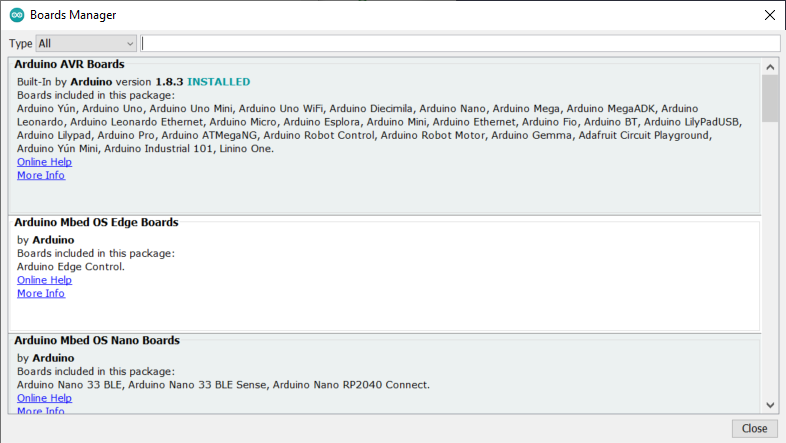
\includegraphics[scale=0.9]{arduinoStart/BoardsManager.PNG}
            \caption{This what the Boards Manager loads up to.}
            \label{fig:boardsManager}
        \end{figure} 
        \item In the search bar, type ``arduino nano connect" (without the quotes)
		\item The first item should be Arduino Mbed OS Nano Boards and should list the Arduino Nano RP2040 Connect.
		\item Move your cursor over it and it should show an Install button. Click it to install the board library.
		\item Wait for it to finish.
		\item While you are waiting, plug your Nano Connect into your computer and let it install it.
		\item As it finished, I received a User Account Control warning asking if I wanted to let dpinst-amd64.exe make changes to my device. I said yes.
		\item Next it asked me if I wanted to install Arduino Universal Serial Bus devices. Again, click to Install.
		\item It popped up again and I clicked Install again. Now it should say that the Arduino Mbed OS Nano Boards has been installed.
		\item Close the Boards Manager.
	\end{enumerate}
\end{enumerate}

\subsubsection{Compiling, Uploading, and Running}
This section can be done on either (or both) computers. The results from one run (between both lab partners)
is needs to be turned in.
\begin{enumerate}
	\item Now go to Files$\rightarrow$Examples$\rightarrow$01.Basics$\rightarrow$Blink.
	\item This will open another window with the Blink program.
	\item Go to Tools$\rightarrow$Board$\rightarrow$Arduino Mbed OS Nano Boards and select the Arduino Nano RP2040 Connect
	\item Go to Tools$\rightarrow$Port and select the COM that isn't COM1 (mine showed up as COM5)
	\item Click the right arrow in the top left of the window to Upload the sketch to the Arduino board.
	\item It should say ``Compiling sketch..." in the lower right and show a progress bar on the lower right.
	\item Then it should switch to Uploading... and finally Done Uploading.
	\item An orange light near the USB port on your board should be blinking.
	\item Congratulations! You have programmed your board!
	\item Now look in the program for the two delay statements. Try changing the values inside the 
          parentheses and re-uploading it. Does the blinking change?
	\item In order to save files and have it portable, you need to change the directory where the 
          Arduino IDE stores it's sketchbooks
	\begin{enumerate}
		\item Go to File$\rightarrow$Preferences
		\item Change the Sketchbook location to your OneDrive and a folder named arduino (lowercase is good)
		\item My OneDrive was in \\C:\textbackslash Users\textbackslash mcneils2\textbackslash OneDrive - Embry-Riddle 
		Aeronautical University\textbackslash arduino
	\end{enumerate}
	\item Now try saving the blink sketch with your changed values.
	\item Demonstrate your working blink and it's storage location to your instructor/TA
\end{enumerate}

\section{USB Demos}
There are two USB demos to show for this lab as well--USB keyboard and USB mouse.
\subsection{USB Keyboard}
\begin{enumerate}
  \item Go to File$\rightarrow$Examples$\rightarrow$USBHID under Examples for 
      the Arduino Nano RP2040 Connect and choose Keyboard. 
  \item This example will type "Hello world" every second forever. 
  \item Modify this to say something pleasant and unique to your lab group 
  \item Modify it to only run once rather than repeated every second (hint: setup vs loop function)
  \item It should now only run once and you get it to run again by pressing the reset button on the 
    Nano Connect (the only button on the actual module).
  \item Demo this to the TA or instructor.
  \item Have a look at the KeyboardModifiers example to think about doing something other than just typing.
  \item As a thought exercise, could you program the board to advance PowerPoint slides every 5 seconds?
\end{enumerate}

\subsection{USB Mouse}
\begin{enumerate}
  \item Go to File$\rightarrow$Examples$\rightarrow$USBHID under Examples for 
      the Arduino Nano RP2040 Connect and choose Mouse. 
  \item This demo moves the mouse arrow between two points around the original location.
  \item Customize the sketch for your lab group.
  \item Demonstrate this to the TA or instructor. 
\end{enumerate}

\section{Other examples}
	Here are some other Examples that might interest you:
	\begin{enumerate}
		\item Basics $\rightarrow$ fade: change the variable led to be LED\_BUILTIN, watch the red/orange LED pulse
%		\item Analog $\rightarrow$ AnalogInOutSerial: change analogInPin to A1 and analogOutPin to LED\_BUILTIN. Turn 
%				the potentiometer (R6) with a screwdriver and watch the LED change accordingly. If you press the magnifying
%				glass button in the top right the actual values will scroll by. You may need to set the baud rate to 9600.
		\item Digital $\rightarrow$ DigitalInputPullup: Change the first pinMode call to use A0 instead of 2. The same for 
				the digitalRead command (2$\rightarrow$A0). Press the right button (SW1) and see the LED blink. 
				 Note that this program isn't written as well as the others since you have to change a number in two
				places. Could you rewrite it better?
	\end{enumerate}

\section{Finishing Up}
  \begin{enumerate}
    \item Create a sketch called \lstinline$getIDs$ using the code at \\ 
        \href{https://github.com/semcneil/CEC325Examples/blob/main/getIDs/getIDs.ino}{https://github.com/semcneil/CEC325Examples/blob/main/getIDs/getIDs.ino}
    \item You will need to install two libraries to make this script run.
    \begin{enumerate}
        \item Go to Sketch$\rightarrow$Include Library$\rightarrow$Manage Libraries 
        \item Install the ArduinoECCX08 and OneWireNG (only version 0.12.2 or earlier) libraries
    \end{enumerate}
    \item Run \lstinline$getIDs$ and submit the results in the end of lab Canvas quiz. The results will be 
                in the Serial Monitor which can be accessed through Tools$\rightarrow$Serial Monitor or the 
                button in the top right of the IDE. It should show 3 IDs for SD18B20 and one crypto serial 
                number. Don't forget that \lstinline$getIDs$ requires two libraries:
        \begin{enumerate}
            \item ArduinoECCX08
            \item OneWireNg version 0.12.x. Version 0.13.x doesn't work
        \end{enumerate}
\end{enumerate}

\section{Turn In}
\begin{enumerate}
    \item Make sure that the TA or instructor has signed off on your modified blink, keyboard, and mouse sketches.
    \item Submit both a PDF of your edited keyboard.ino and the original .ino file of your keyboard sketch. 
            This version of the IDE does not allow printing or saving as a PDF, so you will need to copy the 
            text out of the sketch into something like Word and then save as PDF. Only one 
            submission per group is required but make sure that both your names are on the sketch.
    \item Fill out the end of lab quiz prior to leaving. Note that it includes asking you 
            for the output of the \lstinline$getIDs$ sketch. Both group members should complete
            this quiz.
\end{enumerate}
